V této kapitole představíme v současnosti nejrozšířenější standardy pro
digitální řízení modelové železnice a zařízení, která tyto standardy podporují,
včetně zhodnocení jejich vlastností. Vyhodnotíme, jestli tato zařízení naplňují
požadavky definované v předchozí kapitole.

\section{Digital Command Control} \label{sec:dcc}

Digital Command control (\gls{dcc}) je celosvětově nejrozšířenější systém pro
digitální řízení modelové železnice \cite{dcc_systems:web}. K \gls{dcc} existují
alterntivy, které však v Evropě nejsou prakticky vůbec rozšířené, proto tyto
systémy nebudeme uvažovat.

\gls{dcc} specifikuje komponenty řízení kolejiště a jejich chování – od
doporučeného způsobu zapojení vodičů pod kolejištěm až po komunikační protokoly
a očekávané chování účastníků těchto protokolů. Velkou výhodou je, že \gls{dcc}
je otevřený standard vytvořený organizací \textit{National Model Railroad
Association} (\gls{nmra}), která sdružuje reálné uživatele systému a tedy
reprezentuje reálné jejich skutečné požadavky \cite{dcc_specs:web}.

Princip fungování systému \gls{dcc} ilustruje obrázek \ref{fig:dcc-overview}.

\begin{figure}[ht!]
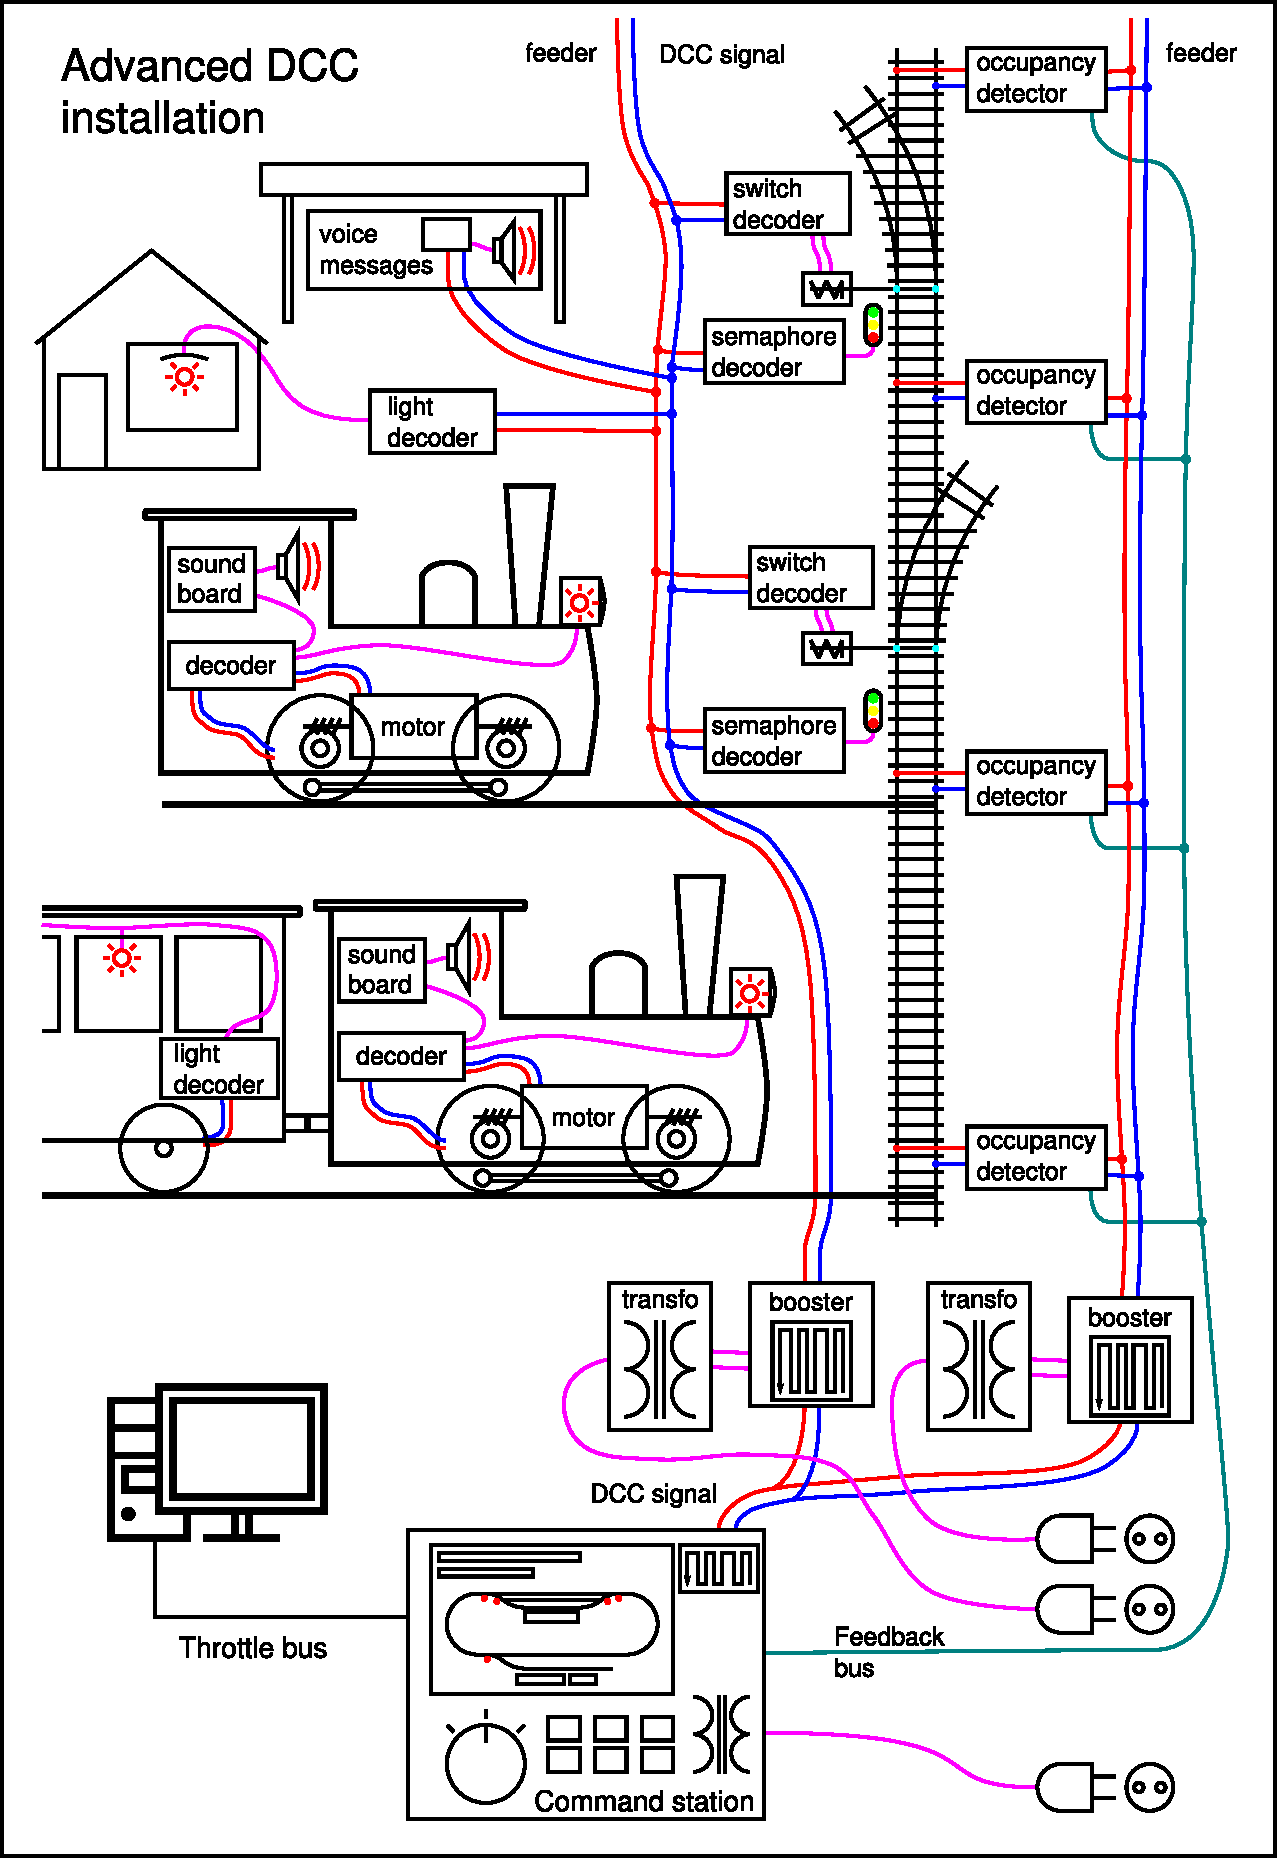
\includegraphics[width=0.95\textwidth]{data/schema_dcc_en.pdf}
\caption{Schéma systému \gls{dcc}. Převzato a upraveno z~\cite{dcc_wikipedia:web}.}
\label{fig:dcc-overview}
\end{figure}

Základním prvkem celého systému je \textit{DCC centrála (Command Station)},
která má 3 hlavní úkoly:

\begin{compactenum}
\item Číst stav \textit{modulů zpětného hlášení (feedback bus)}.
\item Povelovat \textit{dekodéry} lokomotiv, přestavníků, návěstidel apod. To
	centrála provádí generováním \textit{DCC signálu}, do kterého kóduje
	operace požadované po dekodérech – např. \textit{dekodére číslo 541, zastav
	lokomotivu}, \textit{dekodére číslo 4741, aktivuj čelní světla} apod.
\item Obousměrně komunikovat po \textit{sběrnici ovladačů (throttle bus)}.
\end{compactenum}

Zařízení na sběrnici ovladačů interagují přímo nebo nepřímo s operátorem řídím
provoz. Operátor zadává příkazy, například otočením kolečka ovladače, interakcí
s příslušným software apod, tyto příkazy jsou přeposlány do centrály a centrála
je dále přeposílá dekodérům, které přímo vykonávají požadované akce. Centrála
informuje uživatele skrze \textit{sběrnici ovladačů} o změnách ve stavech
vstupů \textit{modulů zpětného hlášení}. Vstupy modulů zpětného hlášení jsou
připojené například k signalizacím obsazení kolejových obvodů, takže uživatel
nebo řídicí SW pozná, že na daném kusu koleje je nebo není nějaký vlak, dále
například ke kontrole koncových poloh výhybek, takže řídicí software je schopen
zabezpečit \textit{vlakovou cestu}.

Pro úplnost uveďme všechny typy vstupů a výstupů, které se v gls{kmz} používají.

Výstupy:

\begin{compactitem}
\item řízení jízdy lokomotiv,
\item řízení osvětlení lokomotiv a vozů,
\item řízení zvuků lokomotiv,
\item nastavení polohy výhybky, výkolejky,
\item rozpojovač,
\item návěstidlo,
\item přejezd,
\item statické pouliční nebo domovní osvětlení,
\item indikace v pultu obsluhy.
\end{compactitem}

Vstupy:

\begin{compactitem}
\item indikace obsazení kolejového obvodu,
\item indikace bodového průjezdu vlaku daným místem skrze infračervené čidlo,
\item indikace koncové polohy výhybky,
\item indikace stavu přejezdu,
\item tlačítka v pultu obsluhy.
\end{compactitem}

Všimněme si jedné klíčové vlastnosti celého systému: pro povelování dekodérů a
pro sběr informací z kolejiště jsou použitý 2 různé sběrnice: \textit{dcc
signál} a \textit{sběrnice zpětného hlášení}. Platí totiž, že signál DCC pouze
jednosměrný. Signál putuje z DCC centrály přes zesilovače skrze 2 kolejnice do
lokomotiv a vozů, které poveluje. Existují jen velice omezené prostředky
jak dostat data zpět z lokomotivy do DCC centrály \cite{railcom}. Tyto
prostředky navíc vznikly až v pozdějších verzích normy \gls{dcc}, takže dnes
nejsou všeobecně zaužívané. Sběrnice \gls{dcc} je tedy fakticky jednosměrná,
dokonce bez kontroly odpovědi dekodérů. To znamená, že centrála musí DCC příkazy
posílat opakovaně, aby zaručila, že je dekodér skutečně přijme. Může se totiž
snadno stát, že lokomotiva zrovna nebude schopna přijímat signál – například
vlivem toho, že se zrovna pohybuje na špinavých kolejích, ze kterých špatně
sbírá. Problém s přijímáním dat vlivem špatného kontaktu se netýká \textit{dekodérů
příslušenství} – na obrázku \textit{switch decoder} a \textit{semaphore decoder}.
Tyto dekodéry jsou připojeny pevným kabelem ke kolejím, takže mají nejlepší
předpoklady dekódovat \gls{dcc} signál korektně. Stále však platí, že dekodér
neodpoví, že přijal a provedl povel. Vykonání povelu mohlo být narušeno čímkoliv
od elektromagnetického rušení signálu až po nepřijetí povelu vlivem chyby ve
firmwaru dekodéru.

Může se zdát, že samotný protokol \gls{dcc} nesplňuje požadavky popsané na
konci kapitoly \ref{chap:nasazeni}. Ačkoliv striktně vzato je tento závěr
správný, je nutné si uvědomit je širší souvislosti. Pří řízení provozu na
modelové kolejišti sledujeme mnohé cíle, z nichž na prvním místě stojí
bezpečnost. I když bezpečnost není zdaleka tak klíčová, jako na skutečné
železnici, materiální škody vzniklé vzniklé například projetím návěsti
zakazující jízdu, vykolejením soupravy, srážky nebo následného pádu na zem
z výšky cca 1 m se mohou pohybovat v řádech desítek tisíců korun. Snad ještě
cennější je osobní časová investice každého modeláře do modelů, které jsou
mnohdy pečlivou ruční prací a které by takovým incidentem mohly být poničeny.
Bezpečnost systému stojí na tom, že nepustíme vlak do míst, kde by mu hrozilo
nebezpečí. K nehodě může dojít v zásadě dvěma způsoby:

\begin{enumerate}
\item \textbf{Vlak stojí a je nesprávně rozjet do místa, které pro něj není
bezpečné.}

	I přes to, že dekodéry nepotvrzují přijetí signálu a provedení akce, této
	situace se jsme schopni vyvarovat. Klíčovým uvědoměním je, že všechny klíčové
	komponenty kolejiště, které řídí směr jízdy vlaku (výhybky, výkolejky) indikují
	svůj stav. To znamená, že když se nepovede provést například přestavení výhybky
	vlivem nedoručení příslušného \gls{dcc} paketu, výhybka se nepřestaví, moduly
	zpětného hlášení správně indikují, že výhybka se nehýbe a řídicí software
	správně vyhodnotí, že nedošlo ke splnění podmínek pro rozjetí vlaku a vlak
	nerozjede.

	Z tohoto pohledu tedy nepotvrzování \gls{dcc} příkazů nevede k nebezpečné
	situaci.

	Jiná situace nastane u dekodérů, které provádějí akce, aniž by indikovaly
	svůj stav. Takové dekodéry jsou například \textit{dekodéry návěstidel}
	(\textit{semaphore decoder} na obrázku \ref{fig:dcc-overview}). Tyto dekodéry
	však nejsou klíčové co se týče bezpečnosti průjezdu vlaku. Špatná návěst
	na návěstidle je nemodelová, ale ke hmotným ztrátám nedojde.
	\footnote{Jiná situace panuje na skutečné železnici, kde návěst návěstidla
	je důležitým komunikačním prvkem mezi dispečerem a strojvedoucím. Je zcela
	klíčové, aby strojvedoucí viděl správnou návěst, protože nesprávná návěst
	by mu mohla povolit jízdu, přestože se například proti němu blíží vlak. Nebo
	by například mohla povolit jízdu vyšší rychlostí, než jaká je v daném
	úseku předepsaná a vlak by pak nemusel stihnout zabrzdit. Proto se na skutečné
	železnici kontroluje, že světly návěstidel, která mají být rozsvícená,
	skutečně prochází proud. Řídicí systém železnice kontroluje, že na návěstidle
	svítí správná návěst.}

\item \textbf{Vlak se nepovede zastavit.}

	Může nastat situace, kdy se vlak blíží k místu zastavení, řídicí software
	mu správně pošle příkaz k zastavení, ale lokomotiva přesto nezastaví.
	Například vlivem již popsaného špatného kontaktu lokomotivy s kolejemi
	a tudíž neschopnosti řádně dekódovat \gls{dcc} signál. Norma \gls{dcc} totiž
	specifikuje \uv{pokud dekodér nedekóduje signál, zůstává ve stejném stavu}.
	Tedy například lokomotiva se pořád pohybuje vpřed.

	Tyto situace v praxi nastávají, ale není v záběru této práce s nimi naložit.
	Tato práce se zaměřuje především na řízení příslušenství a snímání stavu
	kolejiště, nikoliv na řízení jízdy hnacích vozidel.

\end{enumerate}

Závěrem tedy uveďme, že z dosavadního popisu systému \gls{dcc} se zdá, že tento
systém je pro řízení příslušenství vhodný, i když s drobnými nedokonalostmi.

\subsection{Sběrnice zpětného hlášení}

V předchozích odstavcích jsme došli k závěru, že systém \gls{dcc} je v zásadě
vhodný pro řízení příslušenství kolejiště. Vycházeli jsme přitom z předpokladu,
že jsme schopni bezpečně indikovat stav všech prvků v kolejišti. Indikace stavů
probíhá v systému \gls{dcc} skrze \textit{sběrnici zpětného hlášení}
(\textit{feedback bus} ve schématu \ref{fig:dcc-overview}). Prozkoumejme tedy
spolehlivost této sběrnice.

Existuje několik různých \textit{sběrnic zpětného hlášení}
\cite{dcc_feedbacks:web}. \gls{nmra} nedefinuje jednotný standard pro
\textit{sběrnici zpětného hlášení} \cite{dcc_specs:web}, proto různí výrobci
používají různé sběrnice. Uveďme nejpoužívanější sběrnice a jejich vlastnosti.

\subsubsection{S88}

S88 je základní sběrnice zpětného hlášení. Její fungování lze v zásadě
charakterizovat jako \uv{vylepšené posuvné registry} \cite{s88:web}. Jednotlivé
moduly jsou řazeny za sebe, propojují se vždy sousední moduly. První modul
je připojen do \gls{dcc} centrály.

\begin{figure}[ht!]
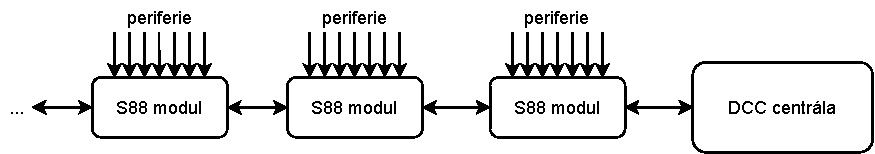
\includegraphics[width=\textwidth]{data/s88.pdf}
\caption{Topologic sběrnice S88.}
\label{fig:s88-topology}
\end{figure}

Tato sběrnice je určena pro low-cost malá kolejiště. Limitujícím faktorem
je především napájení z 5~V, které není vhodné na delší rozvody a malá odolnost
proti rušení \cite{s88:web}.

Jak je patrné z topologie sběrnice, při výpadku (napájení) jednoho modulu
jsou ztracena data i ze všech modulů dále od centrály. Takové chování je pro
profesionální PLC systém nevhodné.

\subsubsection{RSbus}

RSbus je sběrnice firmy \textit{Lenz Elektronik}. Oproti S88 je organizována
do topologie sběrnice. Jednotlivé moduly jsou napájeny samostatně, sběrnice je
dimenzovaná až na 128 modulů, každý s~8 digitálními vstupy \cite{rs:web}
\cite{rs_lib:web}.

\begin{figure}[ht!]
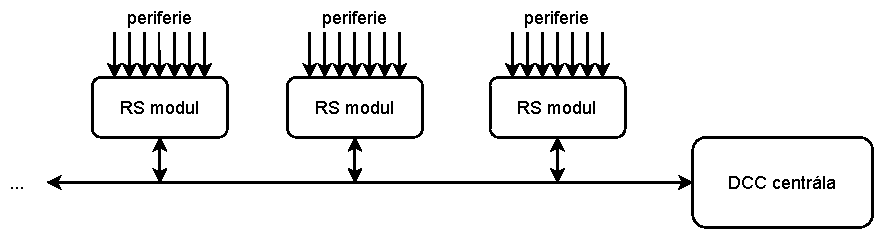
\includegraphics[width=\textwidth]{data/rs.pdf}
\caption{Topologic sběrnice RSbus.}
\label{fig:rs-topology}
\end{figure}

\gls{dcc} centrála řídí komunikaci na sběrnici: posílá výzvy jednotlivým
modulům a moduly odpovídají, pokud mají nějaká data k odeslání. Moduly odesílají
data jen pokud došlo ke změně vstupů, což znamená, že nelze odlišit nefunkční
modul od funkčního modulu, jehož stav vstupů je setrvalý.

Takové chování nesplňuje požadavky definované výše. Pokud by například došlo
výpadku RS modulu a následnému obsazení kolejového obvodu, který tento modul
indikuje, z pohledu řídicího softwaru by byl kolejový obvod stále volný, přesto,
že v obvodu stojí nějaké vozidlo. Řídicí software by pak povolil vjezd vlaku na
úsek, čímž by mohl způsobil srážku vlaků.

K výpadku RS modulu může dojít snadno například ztrátou napájení vlivem chybné
obsluhy, reakce pojistky na přetížení, poruchy apod.

\subsubsection{LocoNET}

Poslední z analyzovaných sběrnic je LocoNET. LocoNET je proprietární sběrnice
společnosti \textit{Digitrax}, jejíž plná specifikace není volně dostupná.
Plné použití této sběrnice podléhá licenčním poplatkům \cite{loconet_license:web}.
Zajímavou vlastnosti sběrnice je, že slučuje sběrnici \textit{throttle bus}
a \textit{feedback bus} (viz obr \ref{fig:dcc-overview}). Řídicí software
v počítači tak může přímo dotazovat moduly zpětného hlášení a úplně tak obejít
DCC centrálu. Sběrnice LocoNET je navíc obousměrná a LocoNET moduly jsou
vstupně-výstupní, takže počítač může přímo povelovat periferie
\cite{loconet:web}.

\begin{figure}[ht!]
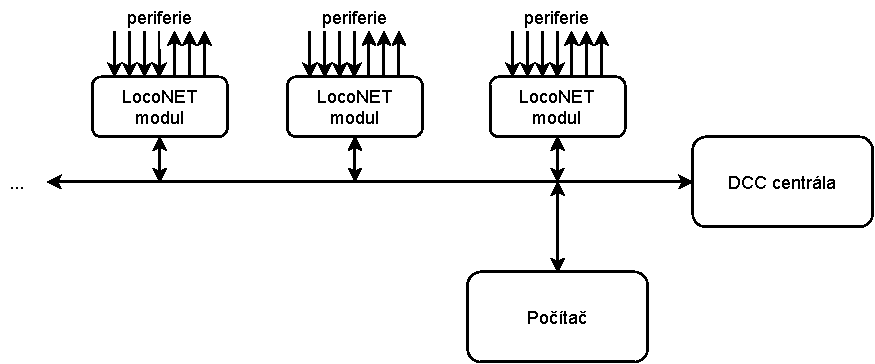
\includegraphics[width=\textwidth]{data/loconet.pdf}
\caption{Topologic sběrnice LocoNET.}
\label{fig:loconet-topology}
\end{figure}

Protokol sběrnice umožňuje dotazovat moduly na jejich stav \cite{loconet-specs},
což umožňuje počítači přímo rozpoznat, které moduly jsou na sběrnici přítomny,
výpadek modulu a oživení modulu po výpadku.

Sběrnice LocoNET splňuje požadavky na bezpečné řízení periferií. Při bližší
inspekci však zjišťujeme, že nasazení této sběrnice by znamenalo nakoupit a
vyměnit cca 100 modulů v kolejišti. Výměna by navíc musela být rozsáhlejší,
LocoNET moduly přímo nepodporují například generování signálu \textit{S-COM}
(TODO ref). Pro nasazení sběrnice LocoNET by musely být instalovány speciální
přídavné moduly pro řízení návěstidel.

\section{Závěr}

V této kapitole byly popsány základní přístupy k řízení moderní digitální
modelové železnice. Bylo zkoumáno, jestli komerční produkty splní požadavky,
které si dala tato práce za cíl. Po vyloučení technicky nezpůsobilých řešení
zbyla sběrnice LocoNET s poznámkou, že její nasazení by bylo poměrně finančně
náročné a pracné.

Při uvažování sběrnice LocoNET jsme narazili na problém s integrací ovládání
návěstidel. Tento problém je obecnějšího rázu: jakékoliv komerční řešení není
schopné nabídnout takovou flexibilitu, jakou bychom v \gls{kmz} potřebovali.
Potřebujeme být schopni integrovat systém řízení kolejiště jeden se současnými
periferiemi, ale i s periferiemi budoucími. Potřebujeme být schopni pružně
reagovat na nové periferie, které přijdou za 10 let.

Uvažme taky aspekt zpětné kompatibility – vlastní systém nám umožní co možná
nejrozumněji zachovat kompatibilitu se stávajícím systémem řízení kolejiště
a minimalizovat tak finanční náklady a čas nutný pro aktualizaci systému.

Vnímejme tuto kapitolu tedy především jako přehled technologií, které se
při řízení současné digitální modelové železnice používají. Přistupme k návrhu,
jak povýšit systém \gls{mtb} výrobou vlastních komponent.

\section{BiDiB}

TODO
